\chapter{UJI COBA DAN EVALUASI}

Pada bab ini dijelaskan tentang uji coba dan evaluasi dari implementasi yang telah dilakukan pada tugas akhir ini.
\section{Lingkungan Uji Coba}
Lingkungan uji coba digunakan untuk uji coba kebenaran adalah salah satu sistem tyang digunakan sistus penilaian daring SPOJ, yaitu kluster \textit{Cube} dengan spesifikasi sebagai berikut :
\begin{enumerate}
	\item Perangkat Keras
	\begin{enumerate}
		\item Processor Intel Xeon E3-1220 v5 (5 CPUs)
		\item Random Access Memory 1536MB
	\end{enumerate}
	\item Perangkat Lunak
	\begin{enumerate}
		\item Kompiler GCC 6.3.0
	\end{enumerate}
\end{enumerate}

Lingkungan uji coba yang digunakan untuk melakukan uji coba kinerja menggunakan komputer pribadi penulis yang memiliki spesifikasi sebagai berikut
\begin{enumerate}
	\item Perangkat Keras
	\begin{enumerate}
		\item Processor Intel® Core™ i7-7500 CPU @ 3.56GHz (4 CPUs), ~3.0GHz
		\item Random Access Memory 8192MB
	\end{enumerate}
	\item Perangkat Lunak
	\begin{enumerate}
		\item Sistem Operasi Windows 10 Education 64-bit
		\item Visual Studio Code
		\item Bahasa Pemrograman C++
		\item Kompiler GCC 7.4.0 (Ubuntu 7.4.0-1ubuntu1~18.04.1) untuk Windows Subsystem Linux
	\end{enumerate}
\end{enumerate}

\section{Uji Coba Kebenaran}
Uji coba kebenaran dilakukan dengan mengirim kode sumber terkait ke dalam situs penilaian daring SPOJ. Berikut bukti hasil pengujian.

\begin{enumerate}
\item Kode sumber dengan metode Multipoint Evaluation (Gambar \ref{fig:verdict_multi})
\begin{figure}[h!]
	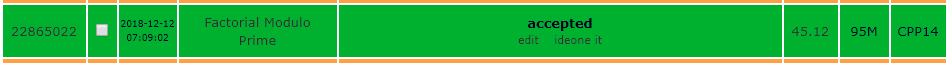
\includegraphics[scale=0.41]{bab5/img/multi-verdict}
	\caption{Umpan Balik Online Judge Metode Multipoint Evaluation}
	\label{fig:verdict_multi}
\end{figure}
\item Kode sumber dengan metode Shifting Evaluation Values (Gambar \ref{fig:verdict_shift})
\begin{figure}[h!]
	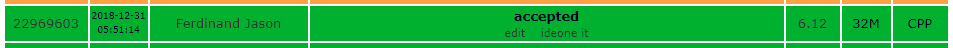
\includegraphics[scale=0.41]{bab5/img/shifting-verdict}
	\caption{Umpan Balik Online Judge Metode Shifting Evaluation Values}
	\label{fig:verdict_shift}
\end{figure}
\end{enumerate}
